\documentclass[10pt,a4paper,twoside, french]{article}
\addtolength{\textheight}{90pt} \addtolength{\topmargin}{-60pt}
\textwidth 164mm \oddsidemargin -2mm \evensidemargin -2mm
\usepackage[utf8]{inputenc}
\usepackage[T1]{fontenc}
\usepackage[english]{babel}
\usepackage{enumerate}
\usepackage{graphicx} 
\usepackage[left=2.5cm,right=2.5cm,top=3.5cm,bottom=3.5cm]{geometry}
%\usepackage{xcolor,rotating,epic,eepic}
\usepackage[font=small,labelfont=bf]{caption}  %% titre dans les minipage
\usepackage{subcaption} %% les sous figure pour les sous legendes
\usepackage{mathtools}   %%   package mathematique
\usepackage{amssymb}  %% symbole mathematique
\usepackage{fancyhdr}  %% pour pied de page et entete et layout
\usepackage{fourier}  %%  police
\usepackage{titlesec}  %% modifier les section
\usepackage{pgfplots} %% provides tools to generate plots and labeled axes easily
\usepackage{color}

\usepackage{tikz}  %%pour les figures
\usetikzlibrary{shapes,arrows,patterns}
\usetikzlibrary{positioning}

\usepackage[colorlinks = true,
            linkcolor = blue,
            urlcolor  = blue,
            citecolor = black,
            anchorcolor = blue]{hyperref} %% permet de renvoyer à la section en cliquant sur la table des matieres
            
            
            
%ecriture des algo
\usepackage{listings}
\lstset{
	language= Matlab,  %choix du language
    frame=tb, % tb=draw a frame at the top and bottom  - single=around
    tabsize=4, % tab space width
    breaklines=true,
    showstringspaces=false, % don't mark spaces in strings
    backgroundcolor=\color{gray!10},
    numbers=none, % display line numbers on the left
%    numbersep=10pt,                   % how far the line-numbers are from the code
%    numberstyle=\normal\color{black}, % the style that is used for the line-numbers
    commentstyle=\color{red}, % comment color
    keywordstyle=\color{blue}, % keyword color
    stringstyle=\color{green}, % string color
    xleftmargin=17pt,
    framexleftmargin=17pt,
    framexrightmargin=0pt,
    framexbottommargin=5pt,
    framextopmargin=5pt,
    escapeinside={(*}{*)}
}
\DeclareCaptionFormat{listing}{\hrulefill\par\vskip1pt#1#2#3}
\captionsetup[lstlisting]{format=listing,singlelinecheck=false, margin=0pt, font={sf},labelfont=bf}
%font={sf}  labelsep=space   %option captionsetup, ,\rule{\dimexpr\textwidth\relax}{0.4pt}

\renewcommand\lstlistingname{Algorithm}  % CHANGER NOM LISTING EN ALGORITHM
%%%%%%%%  Style subsection  %%%%%%%%%%
\usepackage{titlesec}  %% modifier les section
\titleformat*{\section}{\bf}
\titleformat*{\subsection}{\rm}

\numberwithin{equation}{section}
\numberwithin{figure}{section}
\numberwithin{table}{section}

%%%%%%%%%%%  COMMANDE  %%%%%%%%%%%%%%%%%%%%%%%
\newcommand{\vect}[1]{\mathbf{#1}}
\newcommand{\eq}{\Longleftrightarrow}
\newcommand{\chap}[1]{\widehat{#1}}
\newcommand{\bn}{\mathbf{n}}
\newcommand{\bx}{\mathbf{x}}
\newcommand{\R}{\mathbb{R}}
\newcommand{\N}{\mathbb{N}}
\newcommand{\Po}{\mathbb{P}}
\newcommand{\EspAp}[1]{\text{\textbf{#1}}_h}
\newcommand{\enstq}[2]{\left\{#1\mathrel{}\middle|\mathrel{}#2\right\}}
\newcommand{\nm}{|\!|\!|}
\newcommand{\norme}[1]{\left\Vert #1\right\Vert}
\renewcommand{\div}[1]{\text{div } \vect{#1}}
\newcommand{\rot}[1]{\text{\textbf{rot} } \vect{#1}}
\newcommand{\grad}[1]{\text{\textbf{grad} } \vect{#1}}
\newcommand{\diff}{\mathop{ }\mathopen{ }\mathrm{d}}
\newcommand{\restreinta}[1]{\mathclose{}|\mathopen{}_{#1}}
\newcommand{\prodscal}[2]{\left( #1\ ,\ #2\right)}


\begin{document}

\begin{figure}[h]
\centering

\includegraphics[scale=.5]{fig/kth}
\vspace{-1.5cm}
\end{figure}
	\vspace{1cm}    
    \begin{center}
       		\rule{10cm}{1pt} \\[0.6cm]         %% ligne horizontale   \rule[raise-height]{width}{thickness}  
        	{\huge Project \\[0.2cm]
        	\Large An embedded boundary method for the wave \\
        	equation with discontinuous coefficients \\[0.2cm]
         \Large  Numerical analysis for PDE's\\[0.2cm] 
          \large Thomas Frachon - Davoud Saffar Shamshirgar}  \\[0.6cm]
    		\rule{10cm}{1pt} \\[0.5cm]  
	\end{center}    
	
\section{introduction}
The main goal of this manuscript is two present a second order accurate embedded boundary method for a two dimensional wave equation with discontinuous coefficients. The method is based on the Finite difference method with some special treatments to handle the discontinuity at the interface. The method can be used together with the Dirichlet and Neumann boundary conditions. The method discretizes the second order hyperbolic equation directly. Any second order hyperbolic equations can be reformulated to a system of first order PDEs. Different methods have been proposed to treat these systems such as the $h$-Box method by Berger et. al.\ \cite{berger} in the first order formulations. For linear wave propagations, an staggered grid is used, however these type of grids cannot be used simply for any complex boundaries that intersect the grid arbitrarily. 

There exist other methods based on unstructured grids such as Finite volume or Discontinuous Galerkin method to solve the wave equation with jumps in the boundary. Other authors have considered immersed finite element method which is based on the unfitted mesh.

\section{Outline of the algorithm}
We consider a scalar second order wave equation in a two dimensional domain (see figure \ref{...}) with a piecewise constant coefficient,
\begin{align*}
\rho(\bx)=\left\lbrace
\begin{array}{cc}
\rho_I, & \bx\in\Omega_I, \\
\rho_{II}, & \bx\in\Omega_{II}.
\end{array}
\right.
\end{align*}
On each subdomain $\Omega_I$ and $\Omega_{II}$, we consider the solutions $u(\bx,t)$ and $w(\bx,t)$ respectively satisfying the following equations
\begin{align}
u_{tt} &= \dfrac{1}{\rho_I}\Delta u+F(\bx,t), \quad \bx\in\Omega_I,\quad t\geq 0,\\
w_{tt} &= \dfrac{1}{\rho_{II}}\Delta w+F(\bx,t), \quad \bx\in\Omega_{I}I,\quad t\geq 0.
\end{align}
and the initial conditions
\begin{align}
u(\bx,0) &= U_0(\bx),\quad ~u_t(\bx,0)=U_1(\bx), \bx\in\Omega_I, \\
w(\bx,0) &= W_0(\bx),\quad w_t(\bx,0)=W_1(\bx), \bx\in\Omega_{II},
\end{align}
where $F(\bx,t)$ is a forcing term. Now assume a smooth interface $\Gamma$ between the two subdomains such that the solutions $u$ and $w$ match by two jump conditions
\begin{center}
\begin{minipage}[c]{.5\textwidth}
\begin{align}
u &= w, &\bx\in\Gamma, \quad t\geq 0, \\
\dfrac{1}{\rho_I}\dfrac{\partial u}{\partial n} &= -\dfrac{1}{\rho_{II}}\dfrac{\partial w}{\partial n}, &\bx\in\Gamma, \quad t\geq 0.
\end{align}
\end{minipage}
\end{center}

\begin{center}
\begin{minipage}[c]{0.5\textwidth}
\centering
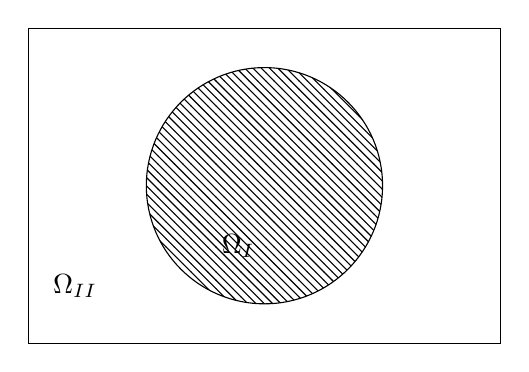
\begin{tikzpicture}
\newcommand{\E}{(-3, -2) rectangle (3,2)}
\newcommand{\A}{(0,0) circle (1.5)}

\draw[fill=white] \E;
\draw[pattern = north west lines] \A;
\draw (-2,-1) node[below left] {$\Omega_{II}$};
\draw (0,-0.5) node[below left] {$\Omega_I$};

\end{tikzpicture}
\captionof{figure}{The Domain is divided into two subdomains $\Omega_I$ and $\Omega_{II}$.}
\end{minipage}
\end{center}

The Laplacian is discretized using a second order accurate approximation given by 
\begin{align}
\Delta_h u_{i,j}^n := \dfrac{1}{h^2}\left( u_{i\pm1,j}^n+u_{i,j\pm1}^n-4u_{i,j}^n\right), \quad \bx_{i,j}\in\Omega_I.
\end{align}
A similar formula can be written for the solution on subdomain $\Omega_{II}$. Moreover we need to define a set of ghost points for the interior subdomain $\Omega_{I}$,
\begin{align}
G_I = \lbrace (i,j), \bx_{i,j}\notin \Omega_I, \text{ but at least one of } \bx_{i\pm1,j}\in\Omega_I \text{ or } \bx_{i,j\pm1}\in\Omega_I\rbrace.
\end{align}
The corresponding expression can be used for the ghost points in $\Omega_{II}$. 














\begin{thebibliography}{0}

\bibitem{berger} 
M.J., Berger, C. Helzel, R.J., LeVeque,
\emph{h-Box methods for the approximations of hyperbolic conservation laws on irregular grids,}
SIAM J. Numer. Anal., 41 (2003), pp. 893--918.


\end{thebibliography}	
	
\end{document}	
